\documentclass{article}
\usepackage{graphicx}
\usepackage{ctex}
\usepackage{listings}


\title{基于K-Means算法的图像分割}
\author{王铭嵩}
\date{\today}

\begin{document}
\maketitle
\section{K-Means算法概述}
\subsection{原理}
K-Means算法是一种无监督分类算法,该算法的任务是将无标签数据集聚类成k个簇,利用贪心策略求得近似解。
具体步骤为:
\begin{enumerate}
    \item 在样本集中随机选取$k$个样本作为初始各簇中心点$\mu_{i}$。
    \item 计算所有样本点与各个簇中心之间的距离,并将其划入最近的簇中。
    \item 根据簇中已有的样本点,重新计算簇中心$\mu_{i}=\frac{1}{|C_{i}|}\sum_{x\in{C{i}}}x$
    \item 重复2,3.
\end{enumerate}
\subsection{优化}
K-Means++优化了各簇中心点的选取:
\begin{enumerate}
    \item 随机选取一个样本点作为第一个簇中心$\mu_1$,
    \item 计算剩余样本点与所有簇中心的最短距离,$D(x^{(i)})=min[dist(x^{(i)},C_j)|j=1,2,...,n]$,某样本点被选为下一个簇中心的概率为$\frac{D(x^{(i)})^2}{\Sigma D(x^{(j)})^2}$,
    \item 重复2,直到选出k个簇中心。
\end{enumerate}
\section{实验过程}
\subsection{图片输入}
输入图片:\\
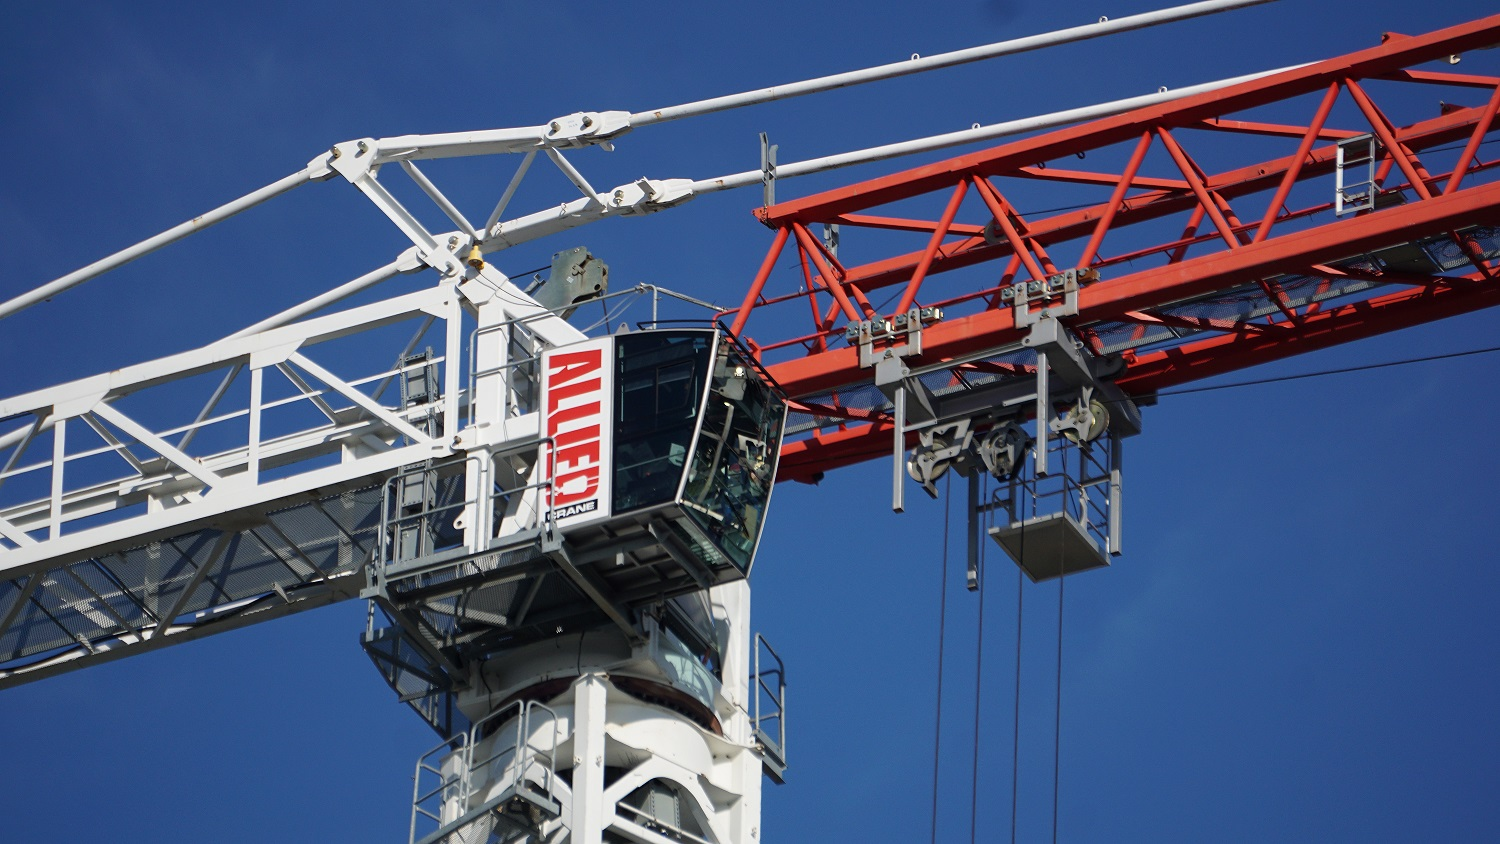
\includegraphics[width=1.0\textwidth]{../python/crane.jpg}\\
已将原始图片的宽高等比缩放之原来的25\%。

\subsection{代码实现}
\textit{仅列出代码实现原理,详细代码请参考源代码。}
\lstset{
    language=python,
    frame=shadowbox,
    breaklines=true
}
imgHandler实现利用pillow库从路径获取图片,并转为二维数组,其中第一维为像素点(按行排列),第二维为RGB信息;RGB信息统一除以255以作归一化处理并转为float类型。返回值为图像原始宽高以及numpy转化过后的二维数组。
\begin{lstlisting}
    # in imgHandler.py:
    def imgToArray(path):
        file=open(path,"rb")
        img=pilImage.open(file)
        imgData=[]
        ...
        return img_width,img_height,np.array(imgData)
\end{lstlisting}
此后利用K-Means++方法的思想来选出k个中心。在Version_1的实现并未利用概率来进行下一个点的选择,而是直接选择距离当前所有聚簇中心最远的点作为下一个点。在后来的评估中认为这么做可能会使某个孤立点单独成簇而缺失掉一个聚簇;
在Version_2的实现中修复了该问题
\begin{lstlisting}
    # in KMeans.py:
    def _getCenterIndex_Center_Dist(data,clusters):
        ...
        return centers,dist_to_centers
\end{lstlisting}
之后进行迭代,每次将所有点归类之离其最近的聚簇中心,并重新计算聚簇的平均值作为下一次迭代的相应聚簇中心。迭代终止条件为迭代数达到目标值或所有聚簇中心的改变(delta)小到某一个特定值。返回值为一个掩码数组,每个位置代表当前像素的所属分组。
\begin{lstlisting}
    # in KMeans.py:
    while epoch<iterations:
        # epoch++
        # updating centers
        # if centers don't change, then break
        # update labels
    return labels
\end{lstlisting}
最后将原始图片的数组配合掩码分别生成对应组的子图片,并存于同一目录下。
\begin{lstlisting}
    # in imgHandler.py
    def arrayToImg(data,mask,path):
        # init img group
        # put pixels
        # generate outputs
    
\end{lstlisting}

\subsection{结果展示}
聚类结果:
\subsubsection{Version=1, clusters=3, iterations=50, delta=0.0001}
实际运行至第9次迭代后输出结果。\\
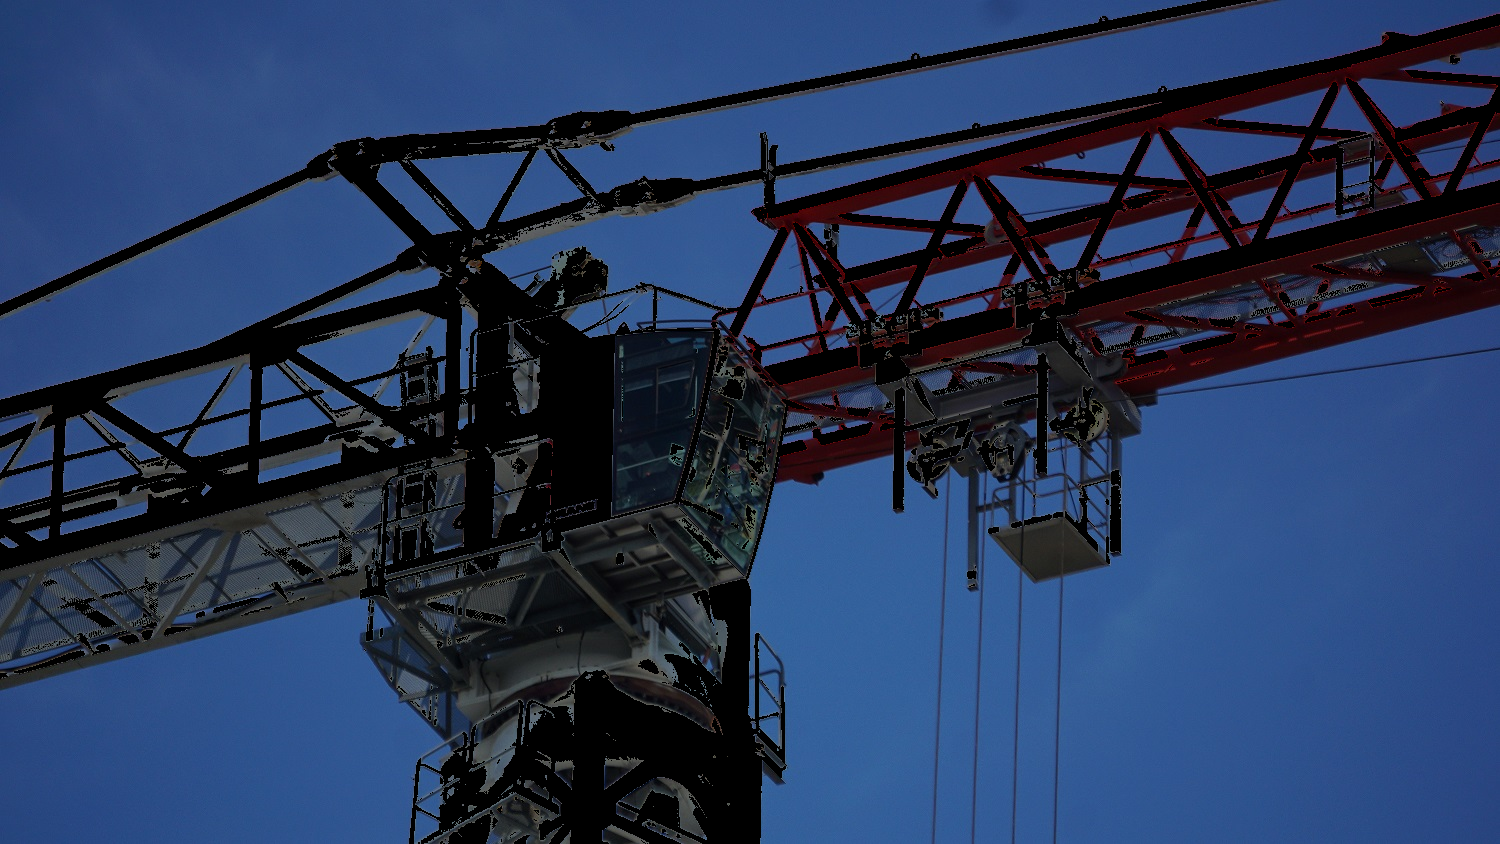
\includegraphics[width=0.33\textwidth]{src/i9d1e-4section1.png}
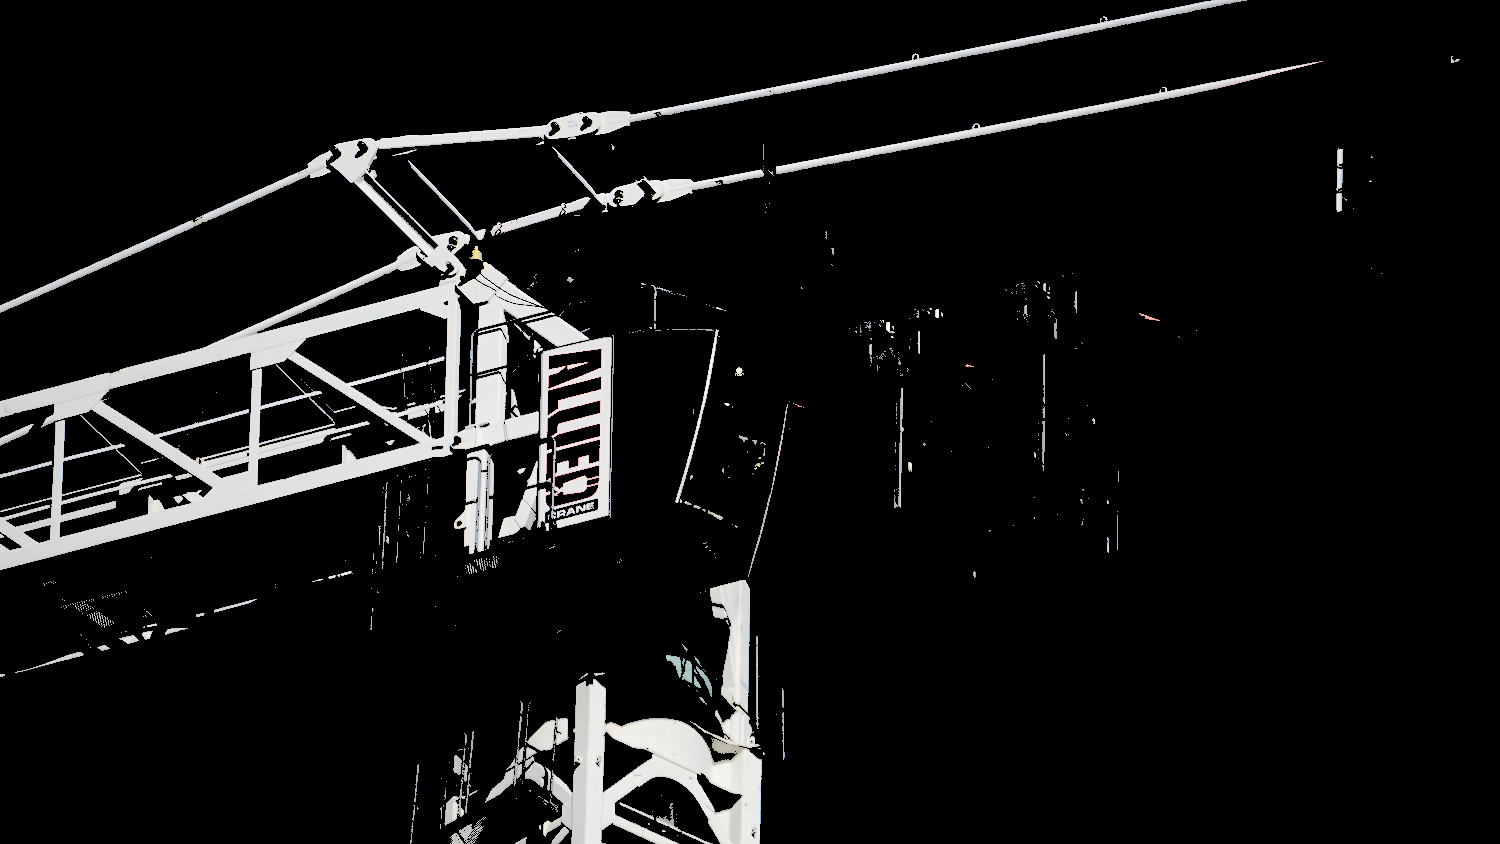
\includegraphics[width=0.33\textwidth]{src/i9d1e-4section2.png}
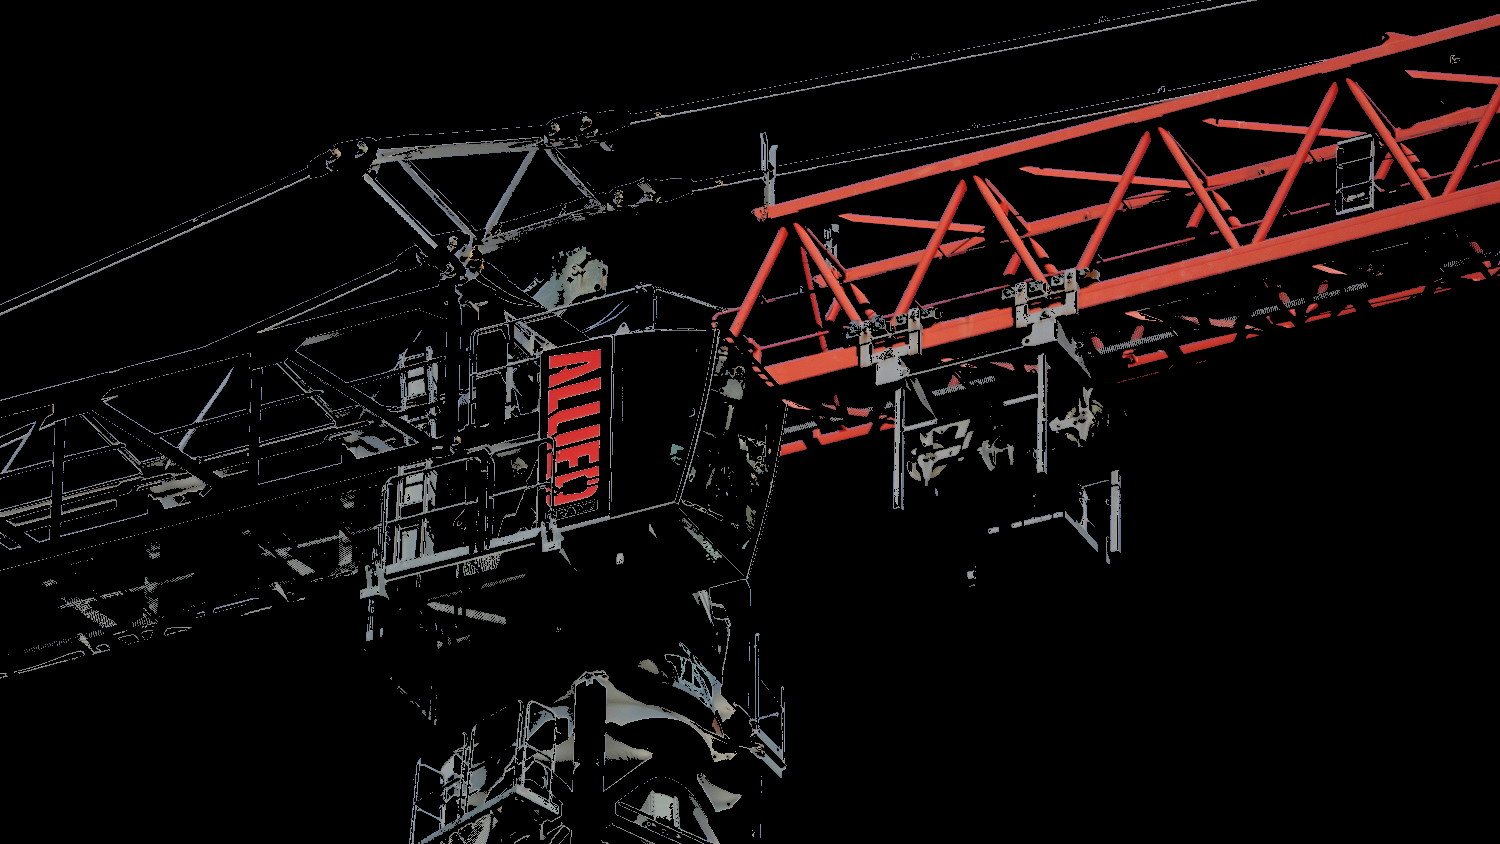
\includegraphics[width=0.33\textwidth]{src/i9d1e-4section3.png}\\

\subsubsection{Version=1, clusters=4, iterations=50, delta=0.00001}
实际运行至第17次迭代后输出结果。\\
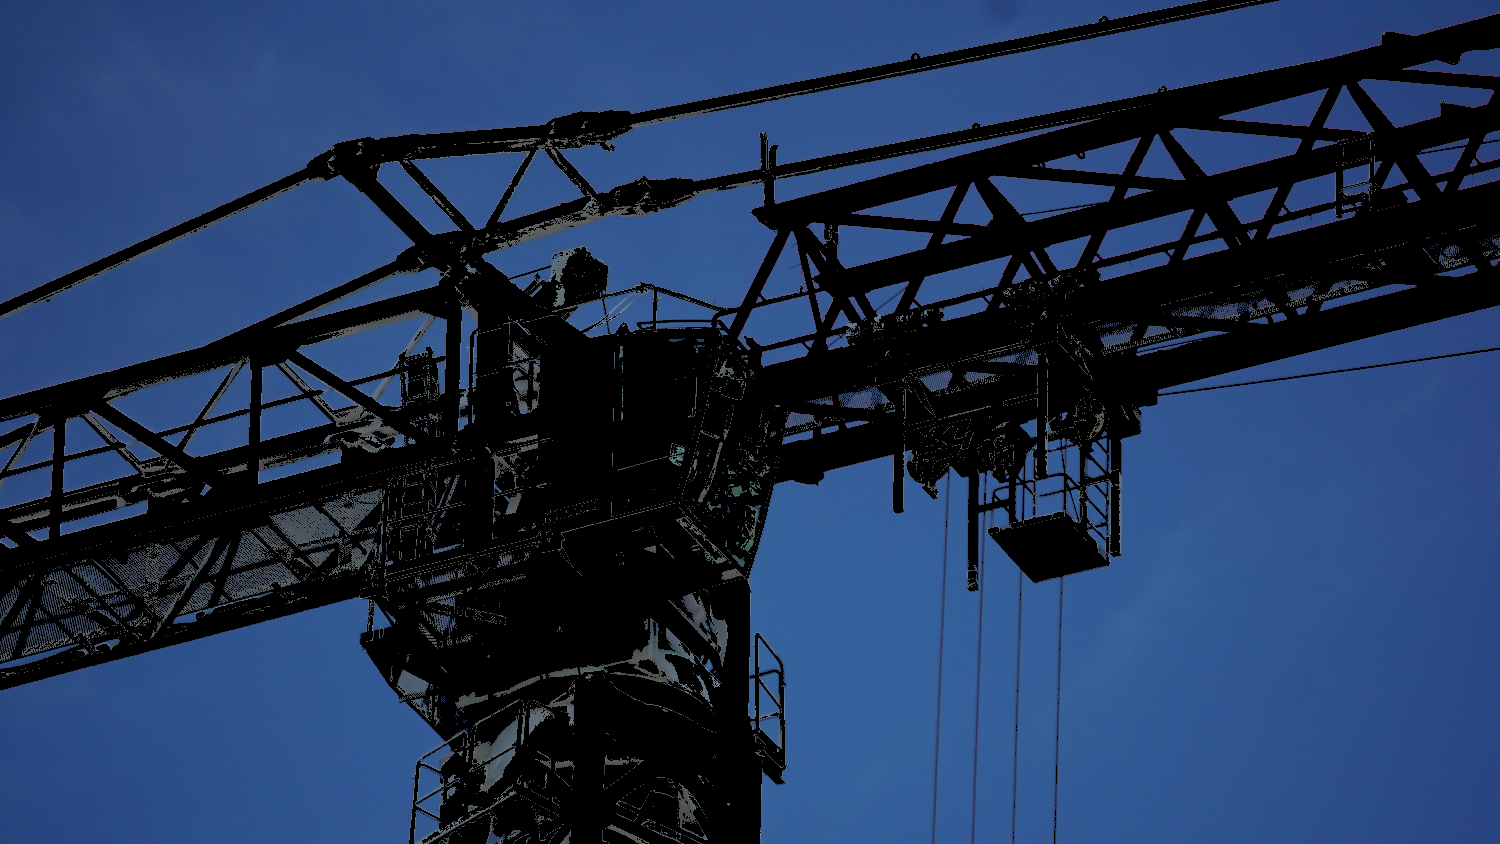
\includegraphics[width=0.5\textwidth]{src/i17d1e-5section1.png}
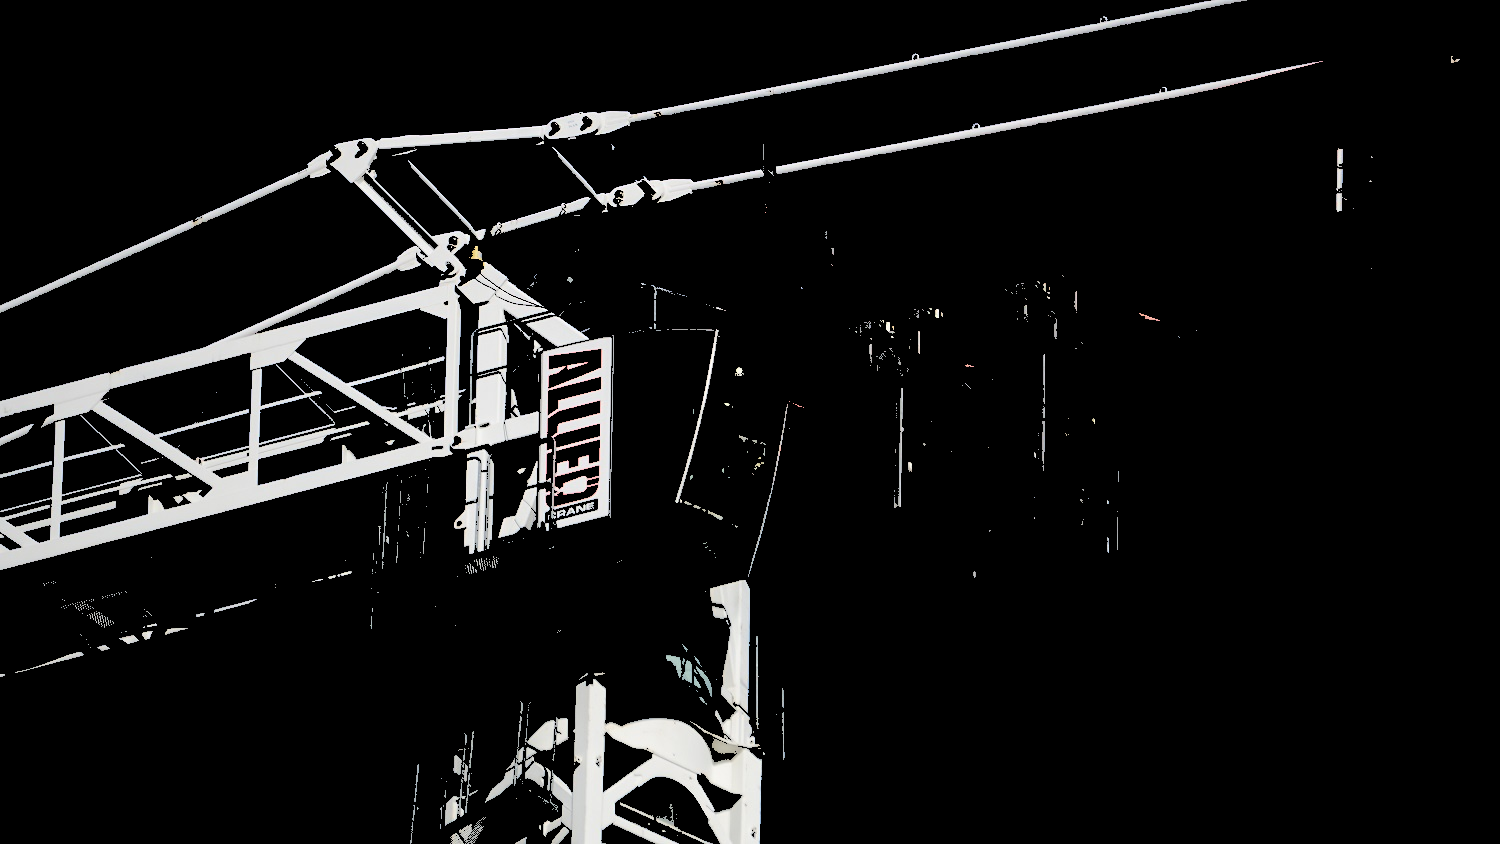
\includegraphics[width=0.5\textwidth]{src/i17d1e-5section2.png}\\
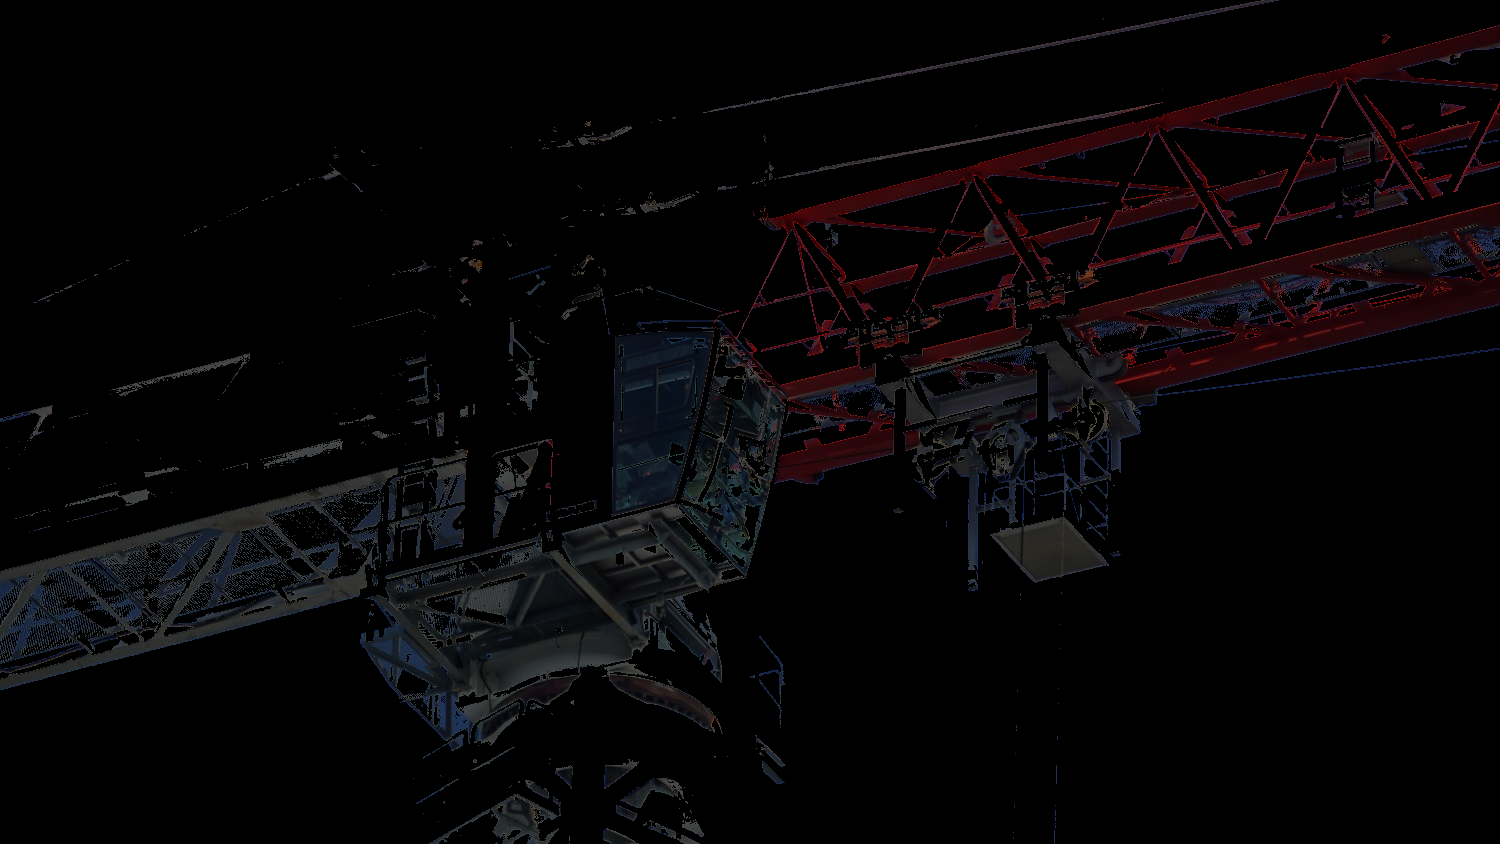
\includegraphics[width=0.5\textwidth]{src/i17d1e-5section3.png}
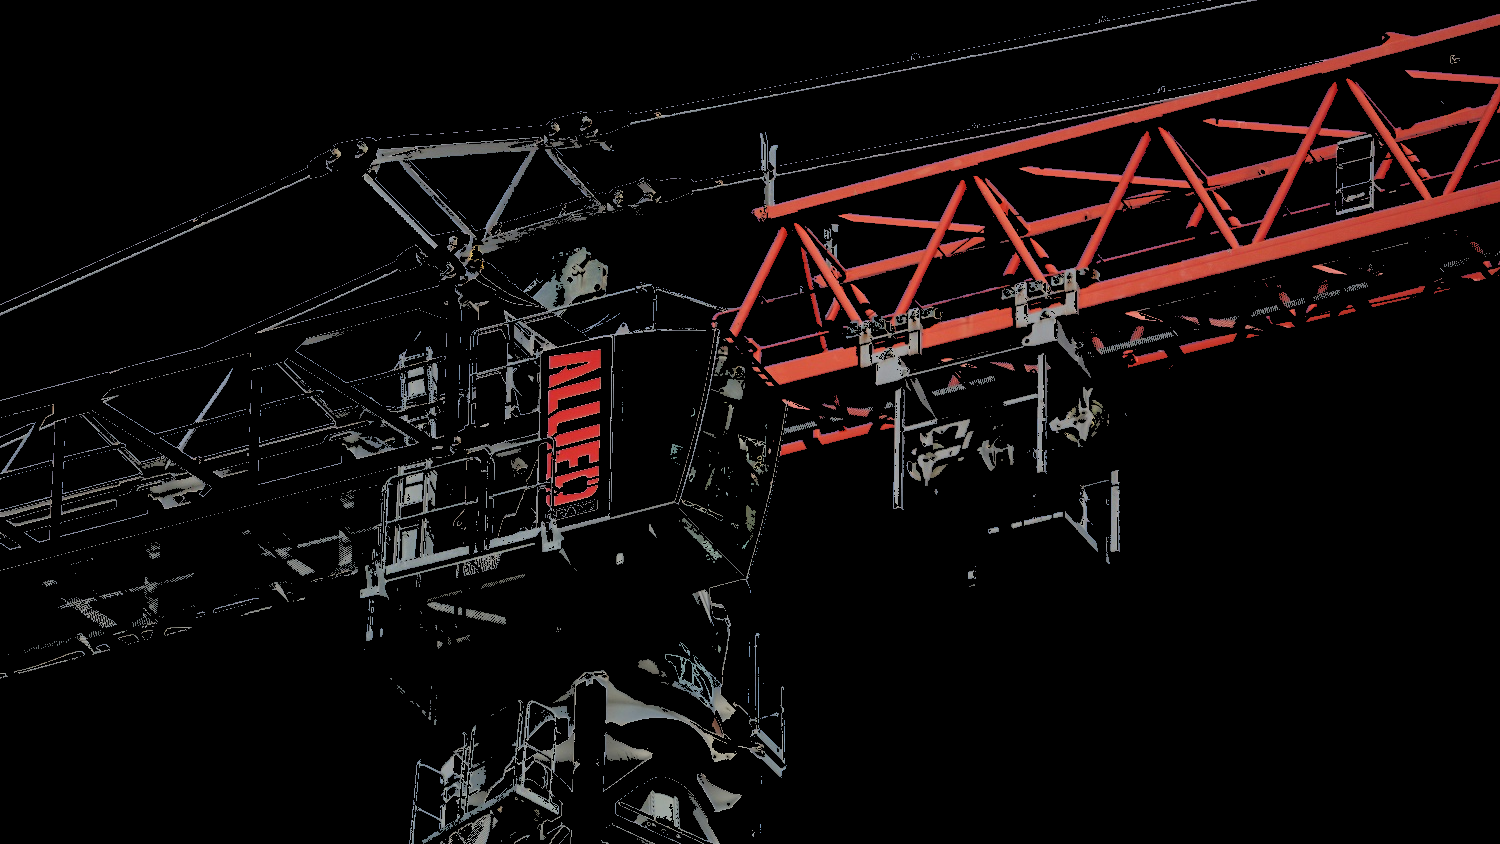
\includegraphics[width=0.5\textwidth]{src/i17d1e-5section4.png}\\

\subsubsection{Version=1, clusters=3, iterations=15, delta=0.0001}
实际运行至第15次迭代后输出结果。\\
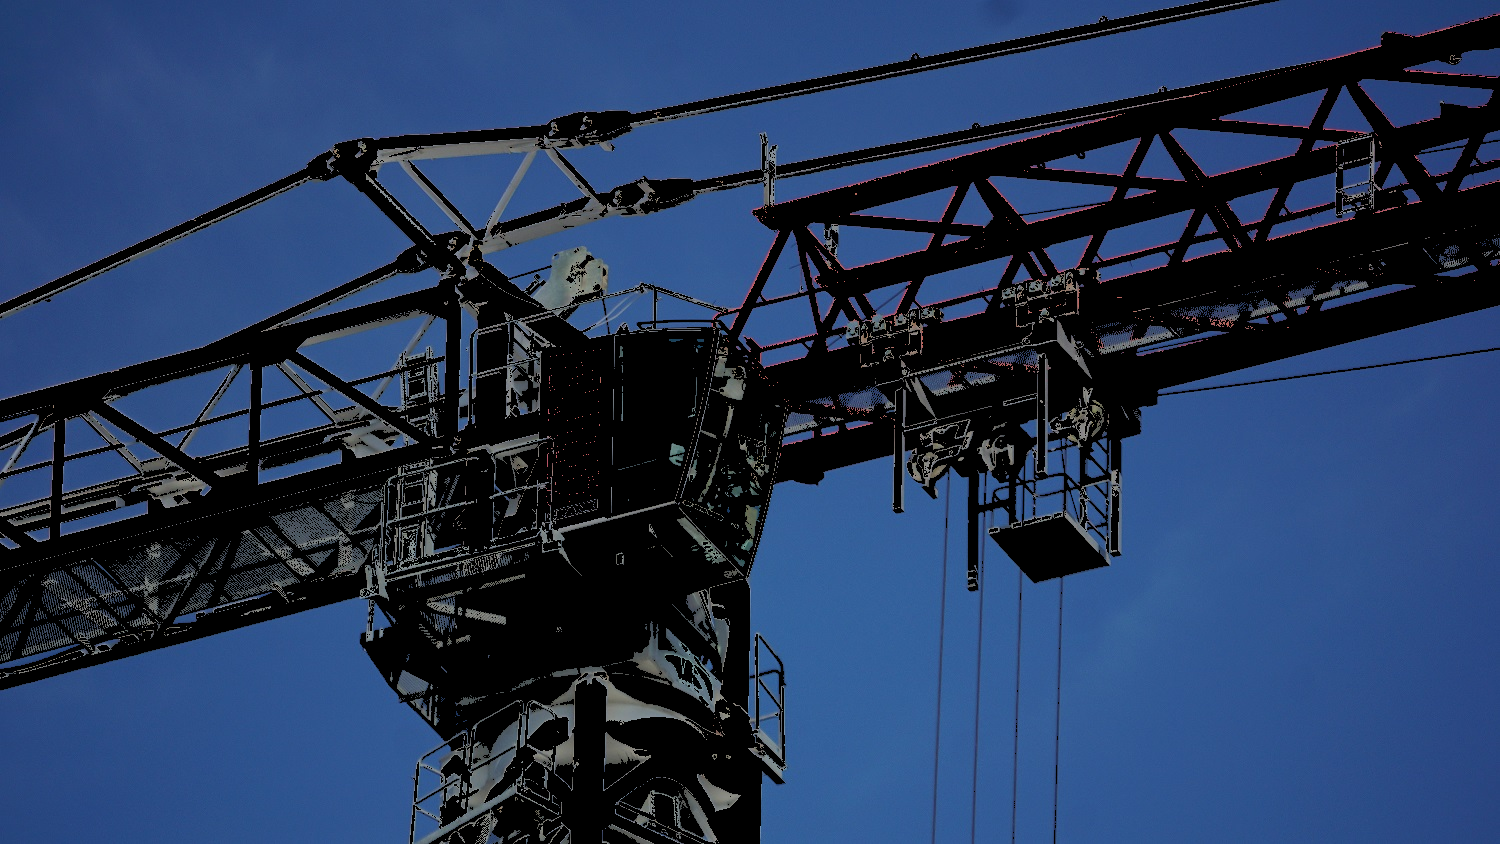
\includegraphics[width=0.33\textwidth]{src/v2_i15d1e-4section1.png}
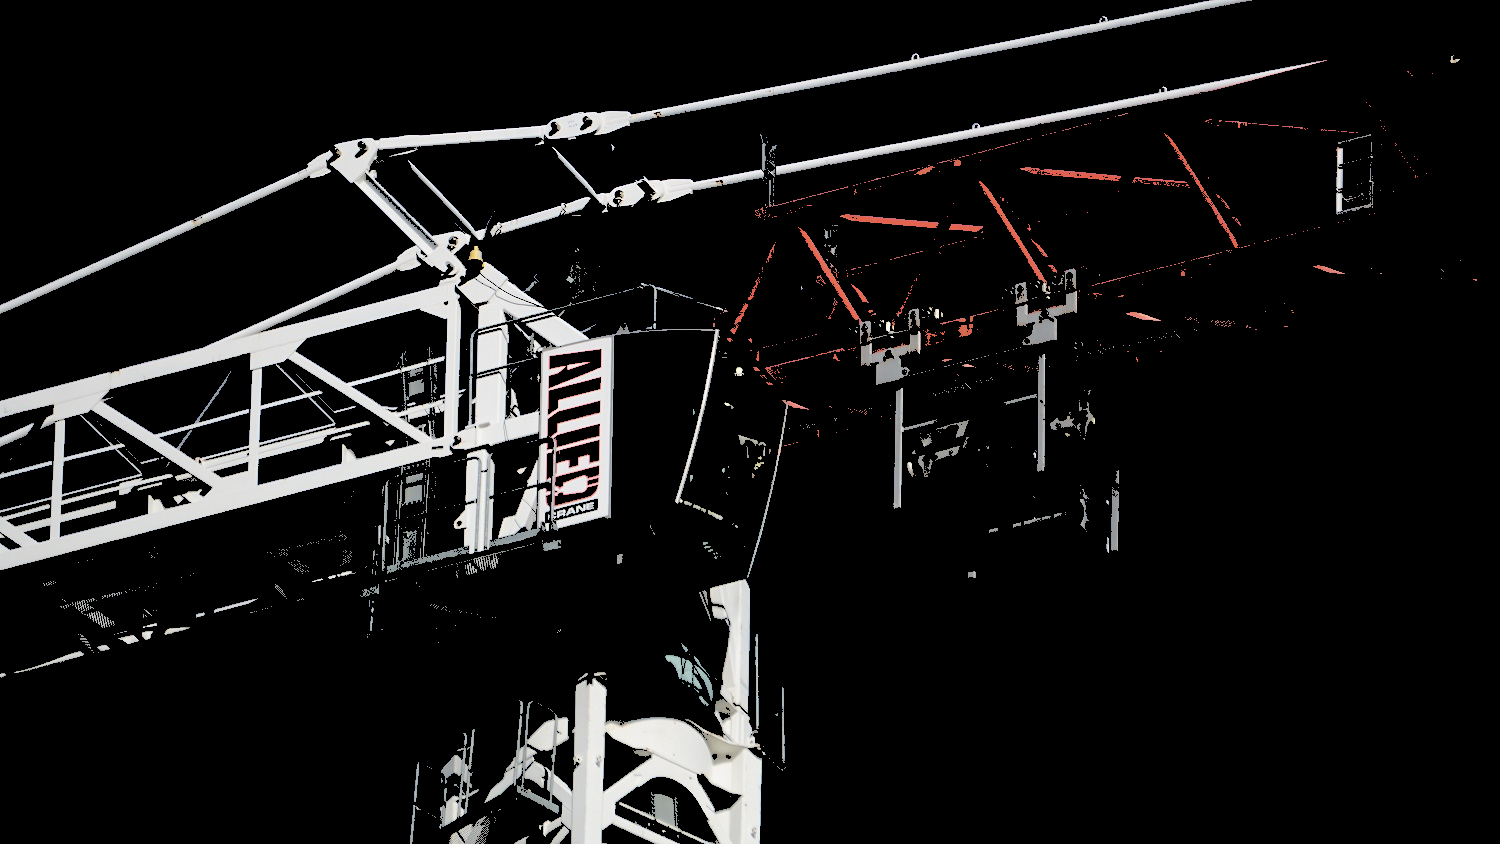
\includegraphics[width=0.33\textwidth]{src/v2_i15d1e-4section2.png}
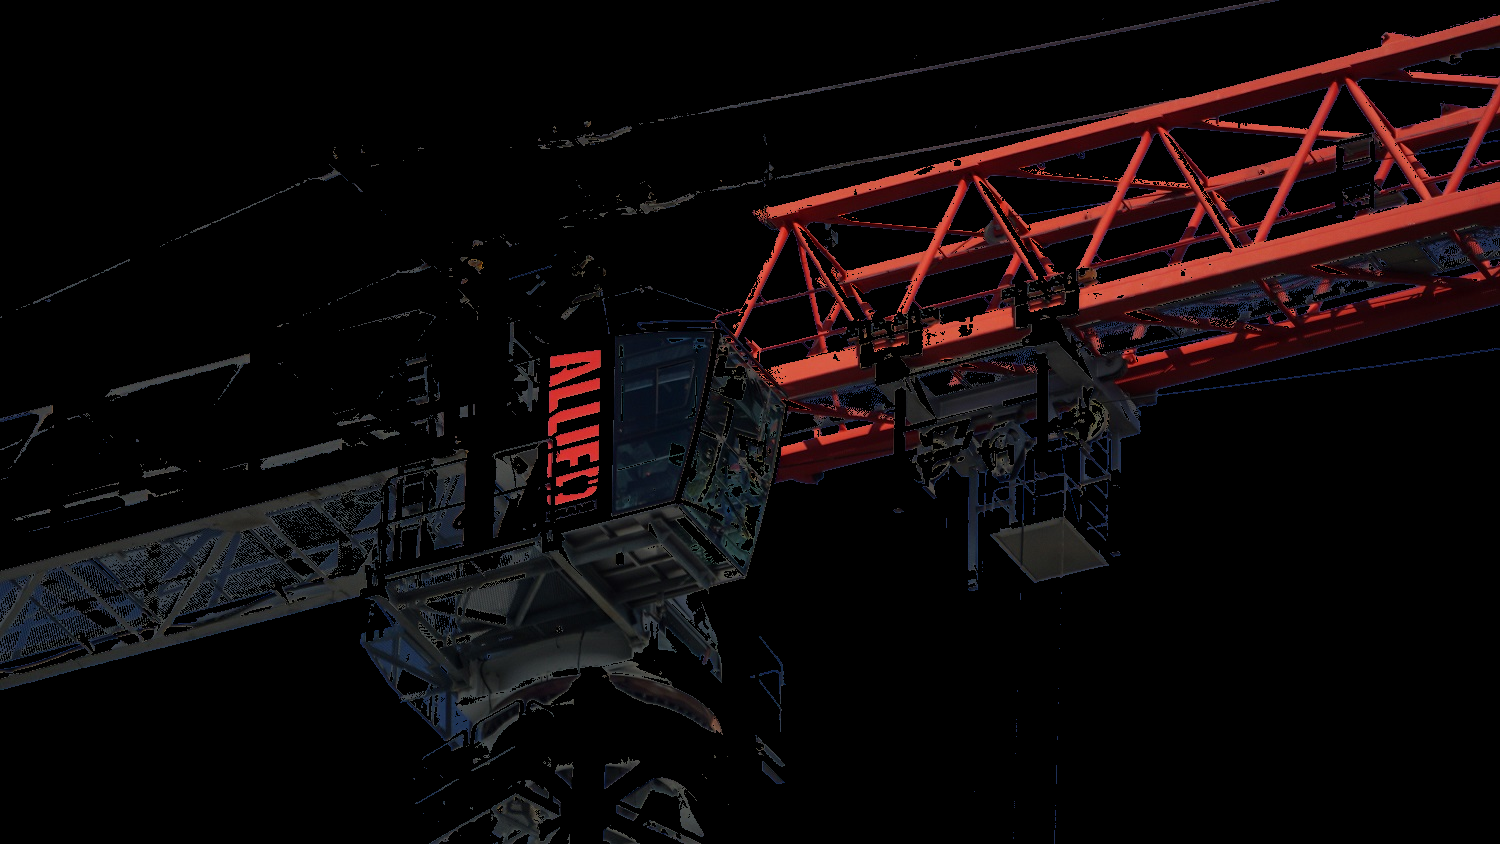
\includegraphics[width=0.33\textwidth]{src/v2_i15d1e-4section3.png}\\
\subsection{问题}
仅将RGB值的相似度作为聚簇依据,而没有考虑图片距聚簇中心的距离的因素。使得分出的类只有数值意义而实际意义不大。
\end{document}